\documentclass[ThesisDJ.tex]{subfiles}

\begin{document}
	Das Projekt zur Evaluation verschiedener Softwarelösungen zur Verbesserung der Kommunikation innerhalb von Teams bzw. Verfahren im Bereich J3 wird zwar im Bereich J3 durchgeführt, hängt aber von keinem der existierenden Projekte, Verfahren oder auch Personen insofern ab, als dass sie direkt als Projektmitarbeiter in das Projekt involviert sind. Somit besteht für die Wahl der Arbeitsweise freie Hand und es ist dem Projektteam überlassen, eine passende Arbeitsweise auszuwählen und in der Folge anzuwenden.\\
	Da der Projektauftrag klar definiert und die zur Verfügung stehende Arbeitszeit durch die Laufzeit stark begrenzt ist, wird weitestgehend traditionell gearbeitet, wobei allerdings Änderungen bzw. weitere notwendige Arbeit nach Bedarf auch nachträglich in die Planung eingebracht werden kann, ohne alle Planungsschritte erneut zu durchlaufen. Einzelne Arbeitsschritte können aber auch agil bearbeitet werden, wenn dies für die Durchführung des Arbeitsschrittes förderlich ist. Zudem werden einige Werkzeuge, wie beispielswiese ein Kanban-Board, verwendet, welche eher dem agilen Projekmanagement zuzuordnen sind. In diesem Sinne handelt es sich um einen 
  traditionellen Projektmanagement-Ansatz mit Verwendung von agilen Methoden. Dieser Ansatz könnte den Vorteil bieten, dass die Planbarkeit des traditionellen Modells erhalten bleibt und um die 
  erhöhte Transparenz, häufiges Feedback während des Projektes und die Kundenorientiertheit eines agilen Modells ergänzt wird \cite[S.~319ff]{dechange_projektmanagement_2024}.
  Eine grafische Darstellung des Arbeitsmodells ist in Abbildung \ref{fig:model} zu sehen.

  \begin{figure}[h!]
    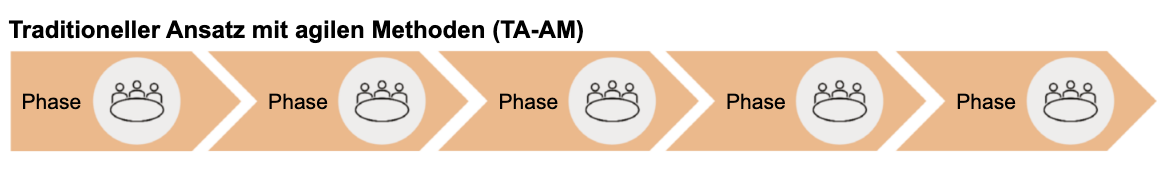
\includegraphics[width=\textwidth]{modell.png}
    \centering
    \caption{Schematische Darstellung des Vorgehensmodells. Entnommen aus \cite[S.~319]{dechange_projektmanagement_2024}}
    \label{fig:model}
  \end{figure}
	
  \subsection{Ausgangslage}
  Die HZD nutzt derzeit eine Mischung aus Skype for Business, E-Mails und der Aufgabenverwaltung in Microsoft Azure DevOps zur Kommunikation \cite{microsoft_azure_nodate}. 
  Dabei treten mehrere Herausforderungen auf, die die Effizienz und Übersichtlichkeit der Kommunikation beeinträchtigen:

  \begin{enumerate}
    \item \emph{Mangelnde Abbildung paralleler Projekte}: Mitarbeiterinnen und Mitarbeiter der Abteilung J3 sind häufig in mehreren Projekten gleichzeitig tätig. Die vorhandenen Kommunikationskanäle unterstützen diese Anforderungen nur unzureichend.
    \item \emph{Redundanz im Informationsfluss}: Nachrichten aus Azure DevOps werden zusätzlich per E-Mail an die betroffenen Personen weitergeleitet. Dadurch entsteht eine Dopplung von Informationen, was die Unterscheidung neuer Inhalte von bereits gelesenen erschwert.
    \item \emph{Unübersichtlichkeit durch getrennte Kommunikationswege}: Skype for Business wird primär für schnelle Nachrichten verwendet. Während die schnelle Reaktionszeit geschätzt wird, empfinden viele Mitarbeitende den separaten Kommunikationskanal als unübersichtlich.
  \end{enumerate}

  Neben der textbasierten Kommunikation wird auch Skype for Business für Videokonferenzen verwendet, insbesondere im Homeoffice oder bei 
  der Zusammenarbeit mit externen Stakeholdern. Dabei ergeben sich weitere Probleme:

  \begin{itemize}
    \item Externe Stakeholder haben oft Schwierigkeiten, an Meetings teilzunehmen, da ein Skype-for-Business-Account erforderlich ist.
    \item Meeting-Einladungen müssen per E-Mail verschickt werden; eine Einladung über den Chat ist nicht möglich.
  \end{itemize}

  Auf Basis dieser Beobachtungen und Schilderungen aus der Praxis lassen sich die zu lösenden Probleme wie folgt zusammenfassen:

  \begin{enumerate}
    \item Es gibt zu viele unabhängige Kommunikationswege innerhalb von Projekten
    \item exteren Stakeholder können nicht effizient in die Prozesse eingebunden werden 
    \item Redundante Verbreitung von Informationen, die die Nachverfolgbarkeit erschwert
  \end{enumerate}

	\subsection{Projektbewertung}
  Das Vorhaben zur Lösung der beschriebenen Probleme ist speziell auf die internen Anforderungen und Rahmenbedingungen der HZD abgestimmt 
  und weist einen klar definierten zeitlichen Rahmen auf. Außerdem soll das Vorhaben in einem fixen Personenkreis bearbeitet werden.
  Damit erfüllt es die formelle Definition eines Projekts als ein einmaliges, zeitlich begrenztes und individuelles Vorhaben,
  welches von einem projektspezifisch organisiertem Personenkreis bearbeitet wird \cite{bronimann_projektmanagement_2022} \cite[S.~5]{dechange_projektmanagement_2024}. 
  Da das Projekt darauf abzielt, einen bestehenden Prozess zu analysieren und durch konkrete Maßnahmen zu verbessern, 
  handelt es sich um ein typisches Prozessoptimierungsprojekt \cite[S.~8]{kuster_handbuch_2022}. Die Kombination aus Problemanalyse und Umsetzung 
  gezielter Verbesserungen entspricht den Merkmalen dieser Projektkategorie. \\

  Die entstehenden Kosten belaufen sich auf die reinen Personalkosten, da keine spezifischen Mittel oder Infrastruktur benötigt werden. Der entstehende
  Nutzen durch eine reibungslosere Kommunikation könnte eine allgemeine gesteigerte Effizienz bei der Umsetzung von Projekten in der Abteilung sein. Basierend 
  auf 

  \subsection{Vorgehensmodell}
  Zur Umsetzung des Projektes stehen mehrere Vorgehensmodelle für das Projektmanagement bereit, welche sich im Laufe der Zeit entwickelt haben. Die Modelle lassen sich in die 
  drei übergeordneten Kategorien \emph{traditionelles Projektmanagement}, \emph{agiles Projektmanagement} und eine Mischung von beiden, dem \emph{hybriden Projektmanagement},
  einteilen. Zur Auswahl eines geeigneten Modells wurde eine Gegenüberstellung der verschiedenen Optionen anhand ihrer zentralen Eigenschaften durchgeführt \cite[S.~405ff]{wysocki_effective_nodate} \cite[S.~15ff]{kuster_handbuch_2022}. Die Ergebnisse sind in 
  Tabelle \ref{tab:methods} zu finden. Aufgrund der Ergebnisse des Vergleichs sowie den Umständen des Projektes wurde sich für ein hybrides Vorgehensmodell entschieden.
  Besonders der Fakt, dass eine klare Anforderungsliste zu Beginn festteht, spricht für die Verwendung von einem traditionellen Ansatz. Um jedoch flexibel in der Bearbeitung zu bleiben ist es sinnvoll,
  agile Methoden zu verwenden. Insbesondere die engmaschige Zusammenarbeit mit Kunden und Stakeholdern, die ein hybrider Ansatz verspricht, ist wünschenswert.

  \begin{table}
    \begin{tabular}{|p{4cm}|p{4cm}|p{4cm}|p{4cm}|}
      \hline 
      Kriterium & Traditionelles PM & Agiles PM & Hybrides PM \\
      \hline
      \emph{Planung} & Detaillierte Vorausplanung, feste Meilensteine & Iterative und anpassungsfähige Planung. Kurzfristig. & Feste Planung mit agilen Teilschritten in einzelnen Aufgaben\\
      \hline
      \emph{Flexibilität} & Sehr gering, Änderungen bringen formale Prozesse mit sich & Hoch - Änderungen sind jederzeit willkommen & Mittel, Änderungen in agilen Teilen gut möglich, ansonsten aufwand durch Formalitäten \\
      \hline
      \emph{Kommunikation} & Fokus auf dokumentenbasierte Kommunikation und ordentliche Meetings & kontinuierlicher Austausch durch bspw. Daily Stand Ups & kontinuierlicher Austausch kombiniert mit ordentlichen Meetings und formellen Dokumenten \\
      \hline
      \emph{Risikomanagement} & Risiken werden zu Beginn identifiziert und formell dokumentiert & Risiken werden kontinuierlich im Projekverlauf erkannt und kurzfristig behandlet & Kombination, bei der initial festgelegte Risiken agil überprüft und angepasst werden. \\
      \hline
      \emph{Anforderungen} & Anforderungen werden anfangs aufgestellt und bleiben stabil. Änderungen erfordern einen formellen Prozess & Iterative Entwicklung, Anforderungen werden stetig angepasst & Grundlegende Anforderungen fest, Änderungen im Detail flexibel \\
      \hline
      \emph{Kundeneinbindung} & Involvierung zu Beginn für die Projektdefintion und am Ende für die Abhnahme & Engmaschige Zusammenarbeit durch Reviews oder Demos, fortlaufendes Feedback & Kundenfeedback in agilen Abschnitten, größere Entscheidungen werden formell geplant \\ 
      \hline
      \emph{Teamstruktur} & Klare Hierarchie mit festen Rollen & Selbstorganisierte, cross-funktionale Teams & Mischung aus fester Hierarchie in der Gesamtorganisation und agilen Teams in einzelnen Phasen \\
      \hline
    \end{tabular}
    \caption{Vergleich der Vorgehensmodelle}
    \label{tab:methods}
  \end{table}
	
	\subsection{Ziele}
  Für das Projekt lassen sich zwei Ziele definieren, die für den erfolgreichen Projektabschluss erfüllt sein müssen.
  Zum einen soll ein Maßnahmenkatalog bis zum 17.03.2025 erstellt werden, welche konkrete Empfehlungen zur Verbesserung der Kommunikation
  enthält. Außerdem soll bis zum 31.03.2025 ein Proof-of-Concept mit Dokumentation bereitgestellt werden, welcher eine exemplarische Umsetzung
  der Maßnahmen darstellt. 

  \subsection{Wahl der Organisationsstruktur}

\begin{figure}[ht]
    \hspace{-0.5cm}
    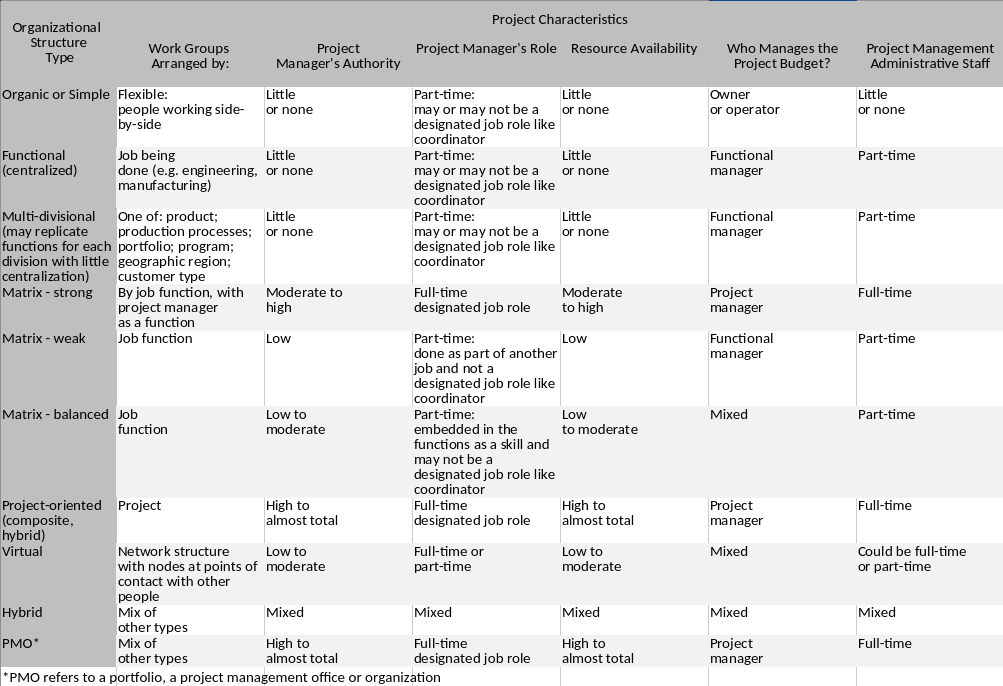
\includegraphics[width=40pc]{./Organisationsstrukturen.png}
    \caption{Typen einer Ogranisationsstruktur. Entnommen aus\cite[S.~75]{PMI2017PMBOK}}
    \label{fig:orgstrukturen}
\end{figure} 

\subsubsection{Beschreibung der Strukturen}

Die in \ref{fig:orgstrukturen} gezeigte Tabelle stellt 10 verschiedene Organisationsstrukturen dar, die für ein Projekt oder eine Unternehmung nach dem "Guide to the Project Management Body of knowledge - PMBOK Guide" eingesetzt werden können.\cite{PMI2017PMBOK} \smallskip\\

\textbf{Organisch oder simpel}\\
In der organischen oder simplen Organisationsstruktur sind die Arbeitsgruppen flexibel organisiert, die Mitarbeiter arbeiten gemeinsam Seite an Seite und die Autorität des Projektmanagers ist sehr gering oder gar nicht vorhanden. Es handelt sich also um eine sehr flache Hierarchie, was sich auch darin zeigt, dass die Rolle des Projektmanagers nur eine Teilzeit-Position ausfüllt und dabei auch nicht zwangsläufig eine eigene Rolle ist.\\
Die Menge an vorhandenen Ressourcen ist hier allerdings sehr gering bis quasi nicht vorhanden und das Budget des Projekts wird vom Eigentümer bzw. Auftrag-geber verwaltet, was auch daran liegt, dass in dieser Struktur kaum bis gar kein Verwaltungspersonal Teil des Teams ist, somit also kein Personal für solche Aufga-ben vorhanden ist. \medskip\\

\textbf{Funktional}\\
Die Funktionale Organisationsstruktur zeichnet sich dadurch aus, dass die Arbeits-gruppen danach gebildet werden, welche Aufgabe ausgeführt wird. Somit können sich die Gruppen auch bei sich verändernden Aufgaben ebenfalls verändern. Da auch in dieser Struktur der Projektmanager wenig Autorität hat, handelt es sich auch hier wieder nur um eine Teilzeitstelle. Es sind wieder wenig Ressourcen vorhanden, im Gegensatz zur organischen Organisationsstruktur wird das Budget allerdings von einem funktionalen Manger verwaltet nicht, mehr vom Eigentümer bzw. Auftraggeber. Ebenfalls gibt es in dieser Struktur Platz für Angestellte mit administ-rativen Aufgaben, wenn auch nur in Teilzeit. \medskip\\

\textbf{Multi-divisional}\\
Die Multi-divisionale Organisationsstruktur ähnelt stark der Funktionalen Organisa-tionsstruktur bzw. baut auf ihr auf. Die Arbeitsgruppen können dabei nach einer Reihe verschiedener Parameter aufgeteilt werden:\\
\begin{itemize}
\item Produktionsprozess
\item Portfolio
\item Programm
\item Geografische Region
\item Art des Kunden
\end{itemize}
Die übrigen Charakteristiken unterscheiden sich nicht von der Funktionalen Organisatzionsstruktur.\\
Damit zeigt sich, dass die Multi-divisionale Organisationsstruktur die Funktionale Organisationsstruktur insofern erweitert, als dass sie die Optionen für die Zusam-mensetzung der Arbeitsgruppen um neue Optionen ergänzt und somit mehrere in sich wieder funktionale Gruppen ermöglicht, die mit nur geringer zentralisierter Ver-waltung zusammen arbeiten. \medskip\\

\textbf{starke Matrix}\\
In der starken Matrix-Struktur sind Arbeitsgruppen nach der Funktion der einzelnen Jobs gruppiert, wobei der Projektmanager eine eine Job-Rolle darstellt. Dabei hat der Projektmanager eine moderate bis hohe Autorität, dementsprechend handelt es sich in dieser Struktur dann auch um eine Vollzeitstelle. Diese Änderung erlaubt dann im Gegenzug eine moderate bis hohe Verfügbarkeit von Ressourcen. Das Budget des Projekts wird ebenfalls vom Projektmanager verwaltet und zur Unterstützung gibt es Vollzeitstellen für adminstrative Mitarbeiter im Projekt.\medskip\\

\textbf{schwache Matrix}\\
Bei der schwachen Matrix-Struktur werden, wie bei der starken Matrix-Struktur die Arbeitsgruppen nach Funktion der einzelnen Jobs aufgeteilt, wobei hier der Projektmanager keine eigenständige Job-Rolle darstellt. Er hat in dieser Struktur auch nur geringen Einfluss und ist nur ein Teilzeit-Posten, der in einen anderen Job im Projekt eingebettet. Dafür sind wieder nur wenige Ressourcen vorhanden und das Budget wird von einem funktionalen Manager verwaltet. Administrative Unterstützung gibt es nur in Teilzeit-Positionen.\medskip\\

\textbf{balancierte Matrix}\\
In der balancierten Matrix-Struktur wird versucht, die Vor- und Nachteile der starken und schwachen Matrix-Strukturen in ein Gleichgewicht zu bringen und ein möglichst gutes Mittelmaß zu finden. An der Anordnung der Arbeitsgruppen ändert sich Nichts, da hierin schwache und starke Matrix übereinstimmen. Die Autorität des Projektmanagers und die Verfügbarkeit von Ressourcen liegen jeweils zwischen den Werten der schwachen bzw. starken Matrix. Der Projektmanager stellt hier wieder nur einen Teilzeit-Posten dar, ebenso wie unterstützende Positionen für administrative Aufgaben, die Zuständigkeit für die Verwaltung des Budgets ist gemischt.\medskip\\

\textbf{Projektorientiert}\\
In der Projektorientierten (auch Komposit oder Hybrid) Struktur sind Arbeitsgruppen nach Projekt aufgeteilt. Der Projektmanager genießt in dieser Struktur nachezu totale Autorität, womit es sich auch um eine Vollzeitposition mit einer Job-Rolle handelt. Dies führt dazu, dass die Verfügbarkeit an Ressourcen ebenfalls nahezu total ist, auch das Budget des Projekts wird vom Projektmanager verwaltet. Bei den administrativen Aufgaben unterstützen ihn Mitarbeiter in Vollzeit-Positionen.\medskip\\

\textbf{Virtuell}\\
Die Virtuelle Struktur stellt die Organisation von Arbeitsgruppen als Netzwerk dar, wobei Knoten die Punkte sind, an denen Mitarbeiter mit anderen Mitarbeitern in Kontakt kommen. Diese Struktur ist besonders für stark verteilte Teams geeignet, in der Mitarbeiter beispielsweise im Home Office getrennt voneinander arbeiten. Der Projektmanager hat hier entsprechend eine niedrige bis moderate Autorität, was sich in der Verfügbarkeit der Ressourcen wiederspiegelt. Durch die starke Verteilung und den gestiegenen Aufwand kann es sich beim Projektmanager trotzdem um einen Vollzeitposten handeln, ebenso wie Positionen für administrative Mitarbeiter. Die Verantwortung für das Projektbudget ist gemischt, kann also von verschiedenen Personen übernommen werden.\medskip\\

\textbf{Hybrid}\\
In der Hybriden Struktur werden, wie der Name es schon vermuten lässt, verschiedene andere Organisationsstrukturen vermischt angewendet, je nach Kombination sind die Charakteristiken also ebenfalls eine Mischung aus den verschiedenen Strukturen.\medskip\\

\textbf{PMO}\\
Ein PMO ist ein Project Management Office bzw. eine Project Management Organization. Das bedeutet, dass in einer solchen Struktur das Projektmanagement für ein Projekt extern übernommen wird und nicht von Mitarbeitenden des eigentlichen Projekts ausgeübt wird. Die Einteilung der Arbeitsgruppen kann dabei ein Mix der anderen Strukturen sein. Der Projektmanager (also das PMO) hat eine nahezu totale Autorität im Projekt, verwaltet das Projektbudget und verfügt über administrative Mitarbeiter, die in Vollzeitpositionen am Projekt arbeiten, dafür die aber die Verfügbarkeit von Ressourcen fast total.

\subsubsection{Auswahl der passenden Struktur fürs Projekt}
Zur Auswahl einer passenden Organisationsstruktur müssen zunächst die Gegebenheiten klar sein. Das Projekt zur Ermittlung einer Software-Lösung zur verbesserten Zusammenarbeit mit Mitarbeitern im Home Office verfügt über keinerlei externe Ressourcen, im Projekt beschäftigt sind drei Personen, dazu ein Auftraggeber, der sich mit den Belangen des Projekts neben den Aufgaben des eigentlichen Jobs beschäftigt.\\
Ein Project Management Office kommt hier nicht in Frage, da das Verhältnis zwischen zusätzlichem organisatorischem Aufwand durch Einbindung einer externen Stelle und dem tatsächlichen Nutzen durch das Projekt nicht gegeben wäre. Darüber hinaus stehen keine Ressourcen zur Finanzierung einer externen Stelle zum Projektmanagement zur Verfügung.\\
Bei einem Projekt mit drei Mitarbeitern erscheint es nicht sinnvoll oder gerechtfertigt, einen dieser Mitarbeiter in Vollzeit für Belange des Projektmanagements abzustellen. Dafür fallen in diesem Bereich nicht genügend Aufgaben an, im Gegensatz dazu müssen in der Ausführung des Projekts die Aufgaben gut aufgeteilt werden. Somit sind Projektstrukturen mit einem Projektmanager als Vollzeitstelle ebenfalls nicht für das Projekt geeignet, wodurch die starke Matrix und die Projektorientierte Struktur ausscheiden.\\
Eine Virtuelle Struktur erscheint ebenfalls nicht sinnvoll, da die Gegebenheiten eines stark individuell verteilten Teams nicht gegeben sind.\\
Die multi-divisionale Struktur ist darauf ausgelegt, mehrere Teil-Teams zu vereinen und in einem größeren Projekt zusammenarbeiten zu lassen. Da die Größe des Projekt-Teams nicht realistisch eine Aufteilung in mehrere Teilprojekte zulässt, ist auch diese Struktur nicht unmittelbar geeignet.\\
Da zu erwarten ist, dass im Rahmen der Durchführung des Projektes die Rollen der Projektmitarbeiter häufig wechseln können, sollte das durch die Organisationsstruktur möglichst gut abgedeckt sein. Da sowohl in den verbleibenden Matrix-Varianten als auch der Funktionalen Struktur Arbeitsgruppen nach dem ausgeführten Job gebildet werden sollen, ist ein solcher häufiger Wechsel hier nicht ideal dargestllt, wohingegen in der Organischen Struktur eine flexible Eintelung und ein Arbeiten Seite an Seite explizit vorgesehen ist.\\
Somit ist die für das Projekt am besten geeignete Organisationsstruktur eine organische bzw. simple Struktur.


  \subsection{Stakeholderanalyse}
  Im folgenden Abschnitt wird eine ausführliche Stakeholderanalyse nach Kuster et al. \cite[S.~86ff]{kuster_handbuch_2022} betrieben, um die sozialen Einflussfaktoren
  auf das Projekt einzuschätzen und im späteren Verlauf ein effektives Stakeholdermanagement durchführen zu können. \\

  Der Auftraggeber ist in diesem Fall ein Stakeholder mit hohem Einfluss und positiver Einstellung. Als Auftraggeber ist er 
  am Erfolg des Projektes interessiert. Er erwartet, dass am Ende die Projektziele erfüllt werden und ein sinnvoller Plan zur Verbesserung 
  der Kommunikation als Endergebnis steht. \\

  Der Bereich J3 ist ein weiterer Stakeholder, welcher für das Projekt von Bedeutung ist. Er ist von den zu treffenden Maßnahmen direkt 
  betroffen, da er die neue Kommunkationsstrategie umsetzen muss. Seine Einstellung ist als neutral zu werten, da er sich zwar eine 
  Ablösung des aktuellen Zustands wünscht, jedoch die neue Lösung von dem Bereich auch akzeptiert werden muss. Es sollten daher aktive 
  Maßnahmen getroffen werden, um sicherzustellen, dass die Akzeptanz für das Projekt und die Ergebnisse hoch bleibt. \\

  Der Leiter der Abteilung J3 kann ebenfalls als Stakeholder gesehen werden, da er ebenfalls Erwartungen an die vorgeschlagenen Lösungen hat.
  Er erhofft sich eine Steigerung und Vereinfachung der Kommunikation im Bereich und daraus auch eine erhöhte Produktivität. Da er für 
  umzusetzende Lösungen sein Einverstängnis geben muss, ist sein Einfluss als sehr hoch anzusehen. Seine Einstellung gegenüber dem Projekt 
  ist als eher neutral zu werten. \\

  Behörden, namentlich die HZD selbst und ihr übergeordnete Behörden wie das Hessische Ministerium für Finanzen oder das Hessische Ministerium 
  für Digitales sind ebenfalls Stakeholder. Durch die Tatsache, dass sie der HZD direkt übergeordnet sind, haben sie einen hohen Einfluss. Dazu 
  ist ihre Einstellung gegenüber dem Projekt als negativ zu bewerten, da organisationsübergreifende Lösungen von ihnen stark bevorzugt werden.
  Im Falle eines möglichen Eingreifens sollte daher vorbereitend geklärt werden, wie man darauf als Projektteam reagiert. \\

  Die Ergebnisse der Stakeholderanalyse sind in Abbildung \ref{fig:stakeholders} als Matrix zusammengefasst.

  \newpage
  \subsection{Stakeholder}
    \begin{figure}[h!]
      \includegraphics[width=\textwidth]{stakeholders.png}
      \centering
      \caption{Stakeholdermatrix des Projekts}
      \label{fig:stakeholders}
    \end{figure}

	
	\subsection{Projektauftrag}
	
	Der Projektauftrag gliedert sich in mehrere Punkte, die im Folgenden beschrieben sind:\bigskip\\
	\textbf{Zielsetzung:}\medskip\\
	Wie bereits im Kapitel zu den Zielen ausführlich beschrieben, bestehen zwei Ziele für das Projekt. Nach einer Evaluation verschiedener Softwarelösungen, die eine Empfehlung für eine der evaluierten Lösungen zum Ziel hat, soll als zweites Ziel die Software, für die eine Empfehlung ausgesprochen wurde ein Proof of Concept aufgesetzt werden, zu dem eine Konfigurationsanleitung für den praktischen Einsatz erstellt wird, die dann vom Bereich J3 verwendet werden kann.\bigskip\\
	\textbf{Vorgehensplan:}\medskip\\
	Als Vorgehensplan wurden initial Meilensteine aufgestellt und mit Terminen versehen, zu denen sie abgeschlossen sein sollten. Diese Meilensteine sowie weitere Details zur Zeitplanung werden im entsprechenden Kapitel näher erläutert.\bigskip\\
	\textbf{Abhängigkeiten und Einflussgrößen:}	\medskip\\
	Wie in der Stakeholdermatrix (Link zu Bild/Kapitel) zu sehen ist, existieren verschiedene Stakeholder, die allerdings alle innerhalb der HZD zu verorten sind. Da es sich beim beschriebenen Projekt um ein Projekt innerhalb des Bereichs J3 handelt, dessen Resultat primär auch nur in diesem Bereich eingesetzt werden soll, werden alle Stakeholder, die außerhalb des Bereichs J3 angesiedelt sind, als externe Stakeholder betrachtet. Dies ermöglicht eine genauere Differenzierung der verschiedenen Stakeholder innerhalb der HZD.\bigskip\\
	\textbf{Personalressourcen und Projektorganisation:}\medskip\\
	Für das Projekt stehen 3 Duale Studenten der HZD im Bereich J3 im Projektzeitraum jeweils einen Tag in der Woche zur Verfügung, es kann also mit 3 Personentagen pro Woche für den gesamten Projektzeitraum gerechnet werden, in der Summe sind das 45 Personentage.
	Aufgrund der sehr kleinen Teamgröße gibt es keinen festen Projektleiter, das Vorgehen und die Aufgabenverteilung werden in gemeinsamen Besprechungen festgelegt und miteinander abgestimmt.\bigskip\\
	\textbf{Schätzung der Projektkosten:}\medskip\\
	Die Projektkosten selbst beschränken sich weitestgehend auf die Personalkosten der Projektmitarbeiter.
	Es muss für das Projekt keine zusätzliche Hardware angeschafft werden, an Kosten für Software fällt gegebenenfalls die Lizenzgebühr für die im Proof of Concept zu betrachtende Software an.\bigskip\\
	\textbf{Rahmenbedingungen und Risiko:}\medskip\\
	Wie bei den Personalressourcen bereits beschrieben ist ein wichtiger Faktor im Projekt die geringe wöchentliche Arbeitszeit am Projekt aller Teammitglieder von einem Arbeitstag pro Woche.\\	
	In der HZD wird aktuell ein Wechsel von Skype zu Webex als Kommunikationsplattform erwogen. Wenn dieser Wechsel erfolgt, könnte die Nutzung einer zusätzlichen Softwarelösung obsolet werden, da mit Webex ein Teil der von der Softwarelösung geforderten Funktionen bereits abdeckt werden und sich der Aufwand, für die verbleibenden Funktionen eine zusätzliche Software zu verwenden gegebenenfalls nicht lohnt. Somit ist ein Wechsel zu Webex ein Projektrisiko, da dadurch das Projektergebnis nutzlos werden könnte. 

	
	\subsection{Dokumentationsform}
  Zur Dokumentation des Projektes und seiner verschiedenen Ergebnisse wird auf die bereits in J3 verwendete Aufgabenverwaltung von Azure DevOps gesetzt.
  Dort werden Vorgänge in einem KanBan-Board hinterlegt, welches über die Reiter \emph{Backlog} \emph{Ready} \emph{In Progress} und \emph{Done} verfügt.
  Dies hat den Vorteil, dass es übersichtlich aufzeigt, an was grade gearbeitet ist und welche Personen dabei involviert sind. Ebenfalls fungieren die 
  Aufgaben als eine Dokumentation, da sie auch nach Erledigung weiter bestand haben und damit der Arbeitsprozess nachvollziehbar bleibt. Außerdem werden 
  Dokumente und Grafiken für das Projekt in der Versionsverwaltung Git gespeichert und auf der Plattform GitHub für alle Mitglieder des Teams bereitgestellt. Dadurch bleibt 
  bei den Dokumenten die volle Änderungshistorie enthalten und alle Teammitglieder können gemeinsam an ihnen arbeiten. Eine beispielhafte 
  Ansicht aus der Aufgabenverwaltung ist in Abbildung \ref{fig:taskmgmt} zu sehen.

  \begin{figure}
    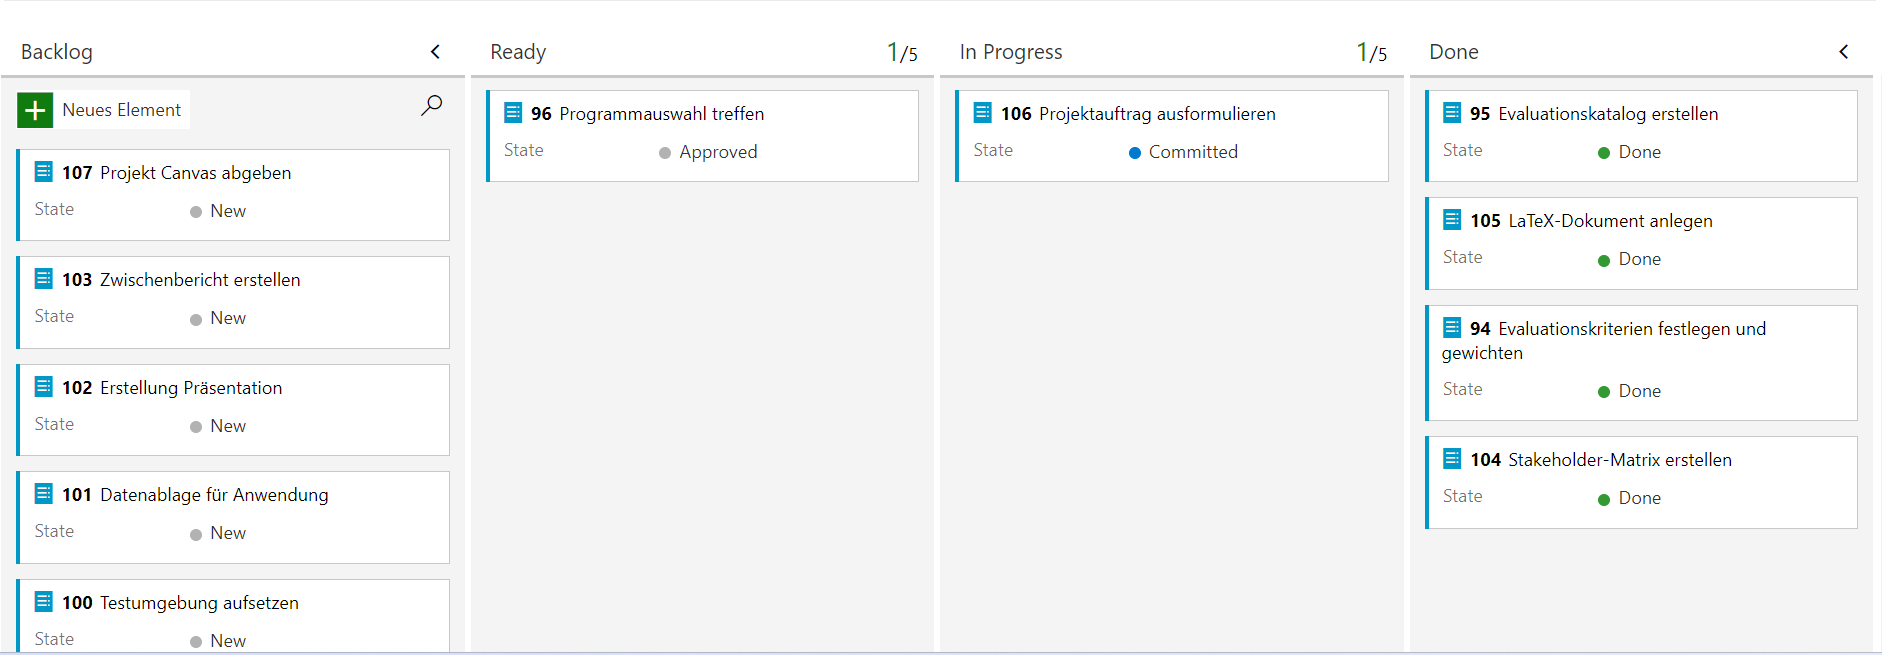
\includegraphics[scale=0.5]{ADO_Board.png}
    \centering
    \caption{Beispielhafte Ansicht der Aufgabenverwaltung}
    \label{fig:taskmgmt}
  \end{figure}
	
	\subsection{Projekt-Canvas}
  \begin{figure}
    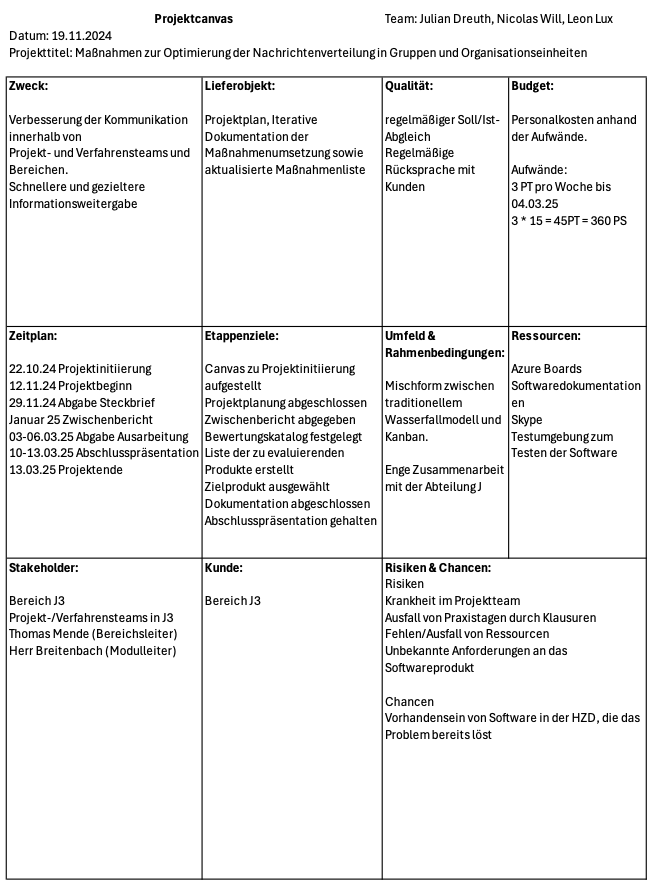
\includegraphics[scale=0.5]{Projektcanvas.png}
    \centering
    \caption{Projektcanvas}
    \label{fig:canvas}
  \end{figure}
  Die Ergebnisse der Projektinitiierung wurden im Projektcanvas \ref{fig:canvas} festgehalten. Dieser stellt damit eine Übersicht über alle relevanten
  Eckpunkte des Projektes zur Verfügung.
\end{document}
